




\section{Feature Extraction and Classification}
\label{sec:feature}



%
%\begin{table}[!b]
%\centering  	
%\vspace{-0mm}
%\caption{{Features extracted in the frame level. }}
%\vspace{2mm}
%\small
%\begin{tabular}{|c|l|}
%    \hline \textbf{Features} & \textbf{Describe}                            \\ \hline
%         $\textbf{p}(t)$  & 3D fingertip position at $t-th$ frame.\\ \hline
%           $d(t)$  & Position difference between adjacent frames.\\ \hline
%           ${{\textbf{v}}}(t)$ &  Velocity of the fingertip motion.       \\ \hline
%         ${\dot{\textbf{v}}}(t)$  & Derived from velocity.  \\ \hline
%          ${{\textbf{D}}}(t)$   & Direction of the fingertip.      \\ \hline
%         $L_f(t)$, $W_f(t)$  & Visible length and width of the finger.\\ \hline       		
%        $\theta_{xy}(t)$, $\theta_{zx}(t)$  & Slope angles at x-y and z-x plane. \\ \hline
%         $\alpha(t)$  &  3D path angle at $t-th$ frame.\\ \hline
%         $\log\frac{1}{\kappa(t)}$  & A notation of curvature of a path.\\ 
%        \hline
%    \end{tabular}
%    \label{tab:features}
%    \vspace{-0mm}
%\end{table}



In this section, we elaborate how to extract features at the frame-, stroke-segment-, and style-levels, respectively (shown in Figure~\ref{fig:featureFlow}). Given a sample, we extract frame-level features (denoted by $f_f^i$ for the $i$-th frame) and then combine the features of $L_{ss}$ consecutive frames to generate a stroke segment-level feature (denoted by $f_{ss}^i$ for the $i$-th stroke segment). After finding the index of the primitive that is closest to each stroke segment, we obtain a  sequence of indices. Then, the occurrences of stroke segment-transition pairs are counted for creating a style-level feature. Then, we discuss the SVM classification for verifying users. 



\begin{table}[!b]
\centering  
\vspace{-3mm}
\caption{{Features extracted in the frame level. }}
\vspace{0mm}
%\small
\begin{tabular}{|l|c|}
    \hline \textbf{Type} & \textbf{Features }                            \\ \hline\hline
     Positions \& Distance & $\textbf{p}(t)$, $d(t)$ \\
        Velocity \& Acceleration & ${{\textbf{v}}}(t)$,  ${\dot{\textbf{v}}}(t)$       \\
        Direction & ${{\textbf{D}}}(t)$          \\
        Finger Size & $L_f(t)$, $W_f(t)$ \\        		
        %Acceleration & ${\dot{\textbf{v}}}(t)$ \\
        Slope angle	\& Path angle & $\theta_{xy}(t)$, $\theta_{zx}(t)$ and $\alpha(t)$\\
        %Path angle & $\alpha(t)$\\
        Log radius of curvature &   $\log\frac{1}{\kappa(t)}$ \\
        \hline
    \end{tabular}
    \label{tab:features}
\end{table}


%==================================================================
%==================================================================
\subsection{Frame-Level Feature}

For a frame $t$, we construct a $19$-dimensional feature vector, which comes from
eight types of kinematics features, as summarized in Table~\ref{tab:features}.  Out of $19$ dimensions, $11$ are provided by Leap Motion directly, and $8$ are calculated.


1) \textbf{Position}.
The 3D fingertip position in the $t$-th frame is denoted as $\textbf{p}(t)= (p_x(t),p_y(t), p_z(t))^T.$
To make the positions among stroke segments comparable, all the fingertip positions within a stroke segment
are normalized by subtracting the fingertip position 
in the first frame of the stroke segment. Thus, the fingertip position
in the first frame of each stroke segment is always $(0,0,0)^T$.
% to-do: component or word?

2) \textbf{Position Difference between Frames}.
The inter-frame position difference is  defined as
$d(t)=\|\textbf{p}(t+1)-\textbf{p}(t)\|.$

3) \textbf{Velocity}.
The velocity of the fingertip motion in the $t$-th frame is provided by the Leap Motion
and we denote it as ${{\textbf{v}}}(t) = ({{v}}_x(t),{{v}}_y(t), {{v}}_z(t))^T.$

4) \textbf{Acceleration}.
The acceleration of the fingertip motion in the $t$-th frame
is derived from the velocity, as ${\dot{\textbf{v}}}(t).$

5) \textbf{Direction}.
The direction of the finger in the $t$-th frame is provided by the Leap Motion
and we denote it as ${{\textbf{D}}}(t) = ({{D}}_x(t),{{D}}_y(t), {{D}}_z(t))^T.$

6) \textbf{Finger Size}.
The visible length and width of the finger in the $t$-th frame are recorded and provided by Leap Motion and we denote them as  $L_{f}(t)$
and $W_{f}(t)$, respectively.
% We normalize these two feature values such that each of them conforms to a standard Gaussian distribution based on all the collected data.

7) \textbf{Slope Angle}.
The slope angles at the $t$-th frame are defined as
\begin{align}  \scriptsize
\theta_{xy}(t)=\arctan\frac{{\dot{p}}_y(t)}{{\dot{p}}_x(t)},\notag  \; \\ \notag
\theta_{zx}(t)=\arctan\frac{{\dot{p}}_x(t)}{{\dot{p}}_z(t)}. \notag
\end{align}


8) \textbf{Path Angle}.
Path angle $\alpha(t)$ is the angle between lines $\textbf{p}(t)\textbf{p}(t+1)$ and $\textbf{p}(t-1)\textbf{p}(t)$,
as shown in  Figure~\ref{fig:curvature}.


9) \textbf{Curvature}. As show in Figure~\ref{fig:curvature},
we calculate the log radius of curvature,  $\log \frac{1}{\kappa(t)}$, at the $t$-th frame as one feature,  where $\kappa(t)$ is the curvature:
\vspace{-0mm}
$$
\kappa(t)=\frac{\sqrt{c_{zy}^{2}(t)+c_{xz}^{2}(t)+c_{yx}^{2}(t)}}{({\dot{p}}(t)_x^{2}+{\dot{p}}_y^{2}(t)+{\dot{p}}_z^{2}(t))^{3/2}}, $$
and
$$c_{zy}(t) = {\ddot{p}}_z(t) \times {\dot{p}}_y(t)-{\ddot{p}}_y(t) \times {\dot{p}}_z(t). $$
%\vspace{-2mm}


%
%\subsection{Frame-Level Feature}
%
%For a frame $t$, we construct a $19$-dimensional feature vector, which comes from
%eight types of kinematics features, as summarized in Table~\ref{tab:features}.  Out of $19$ dimensions, positions, velocity, direction and finger sizes are provided by Leap Motion directly, and other $8$ dimensions are calculated. We normalize each dimension of these features such that it conforms to a standard Gaussian distribution in each word.


We normalize the feature data in each dimension  such that it conforms to a standard Gaussian distribution in each word. \jingap{Specifically, we first calculate a mean value and its standard deviation. Then the values are converted to new values that fit into a standard Gaussian distribution.}
%\jing{ We further group several adjacent frames' features into a stroke segment-level feature to compare the similarity between writing components.}


\begin{figure}[!t]
\centering
\vspace{-10mm}
\begin{tabular}{c}
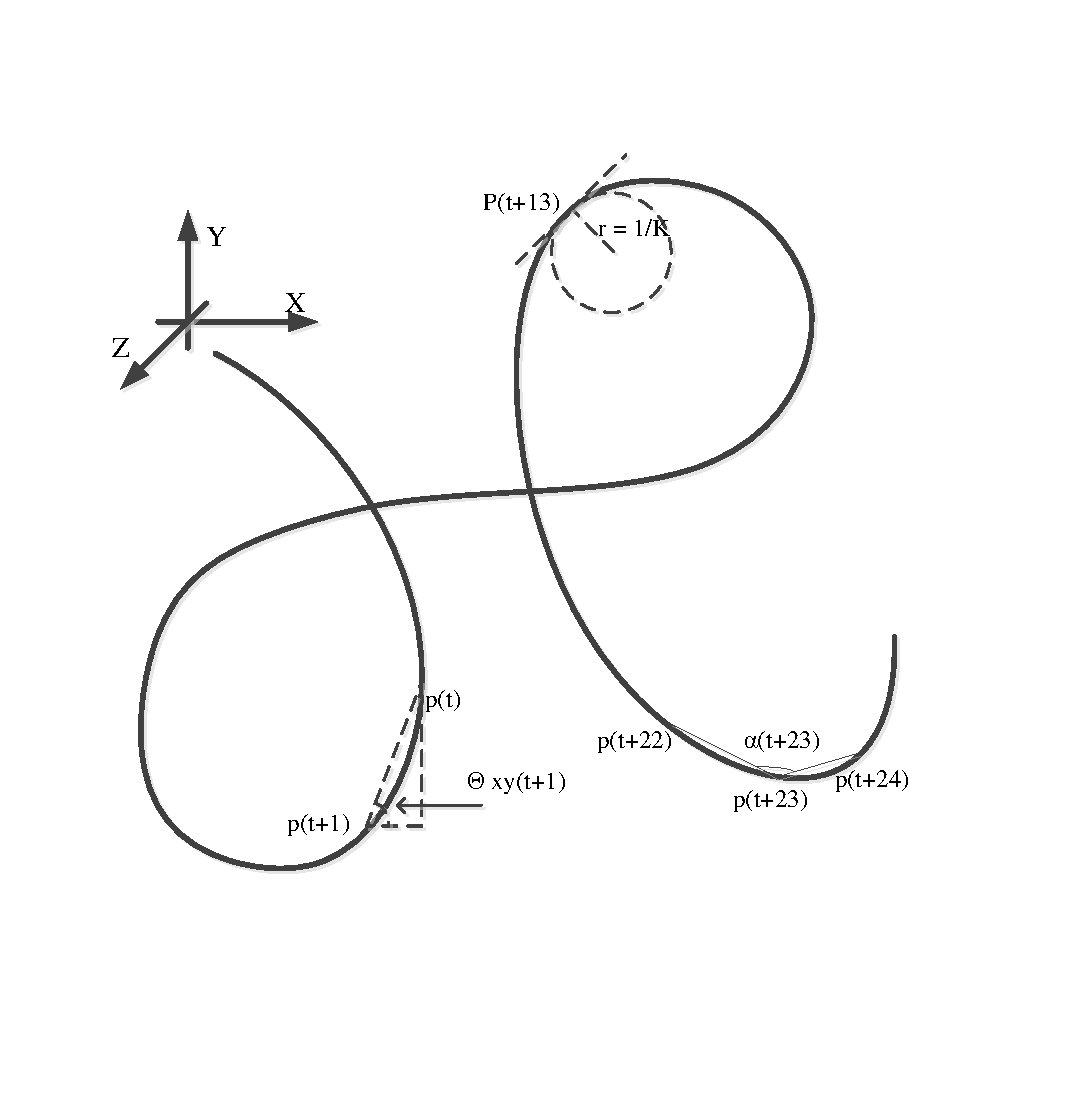
\includegraphics[width=0.9\columnwidth]{./Graphic/Pictures/slopeangle.pdf}
\end{tabular}\vspace{-18mm}
\caption{{\jing{An illustration of slope angle, path angle and curvature.}} \vspace{-2mm}}
\label{fig:curvature}
\end{figure}




%\begin{figure}[t]
%\scriptsize
%\centering
%\vspace{-0mm}
%\begin{tabular}{ccc}
%
%{\includegraphics[width=0.22\columnwidth]{./Graphic/Pic_words_forSystemSection/11_thWord_component.eps}\vspace{-0mm}}
%&{\includegraphics[width=0.22\columnwidth]{./Graphic/Pic_words_forSystemSection/111_thWord_component.eps}\vspace{-0mm}}
%&{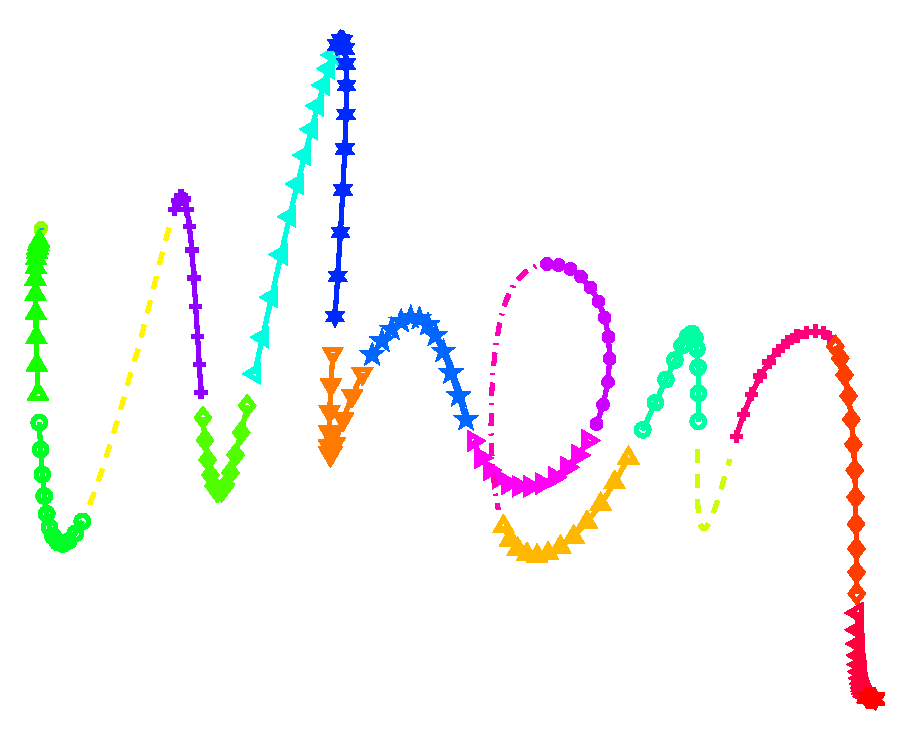
\includegraphics[width=0.22\columnwidth]{./Graphic/Pic_words_forSystemSection/1111_thWord_component.eps} \vspace{-0mm}} \\
%\multicolumn{3}{c}{(a) Extracted components for the word `when' } \\ 
%\multicolumn{3}{c}{ } \\ 
%{\includegraphics[width=0.22\columnwidth]{./Graphic/Pic_words_forSystemSection/22_thWord_component.eps}}
%&{\includegraphics[width=0.22\columnwidth]{./Graphic/Pic_words_forSystemSection/222_thWord_component.eps}}
%&{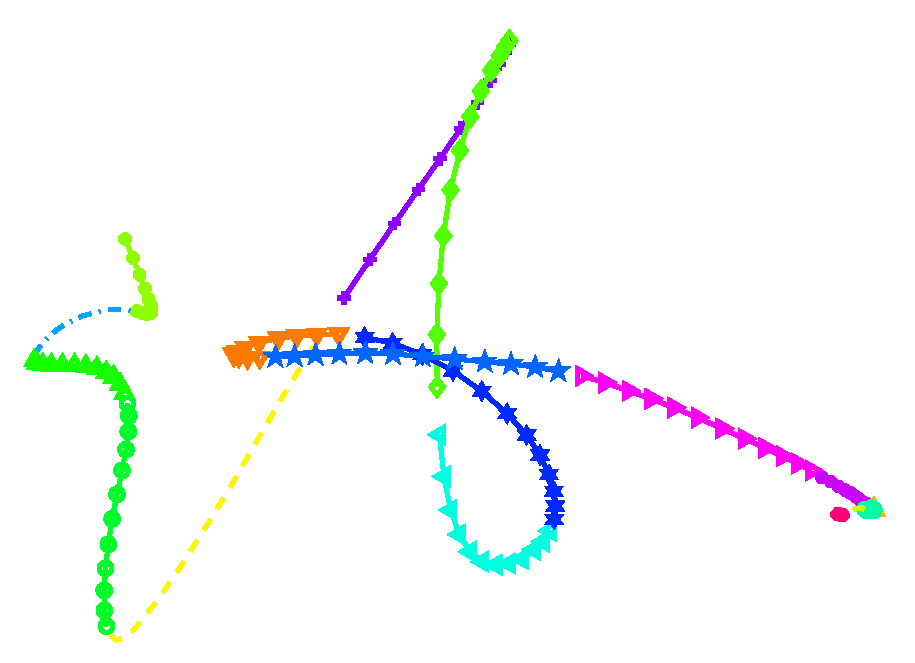
\includegraphics[width=0.22\columnwidth]{./Graphic/Pic_words_forSystemSection/2222_thWord_component.eps}} \\
%\multicolumn{3}{c}{(b) Component extraction for word `it'} \\ 
%\multicolumn{3}{c}{ } \\ 
%{\includegraphics[width=0.22\columnwidth]{./Graphic/Pic_words_forSystemSection/33_thWord_component.eps}}
%&{\includegraphics[width=0.22\columnwidth]{./Graphic/Pic_words_forSystemSection/333_thWord_component.eps}}
%&{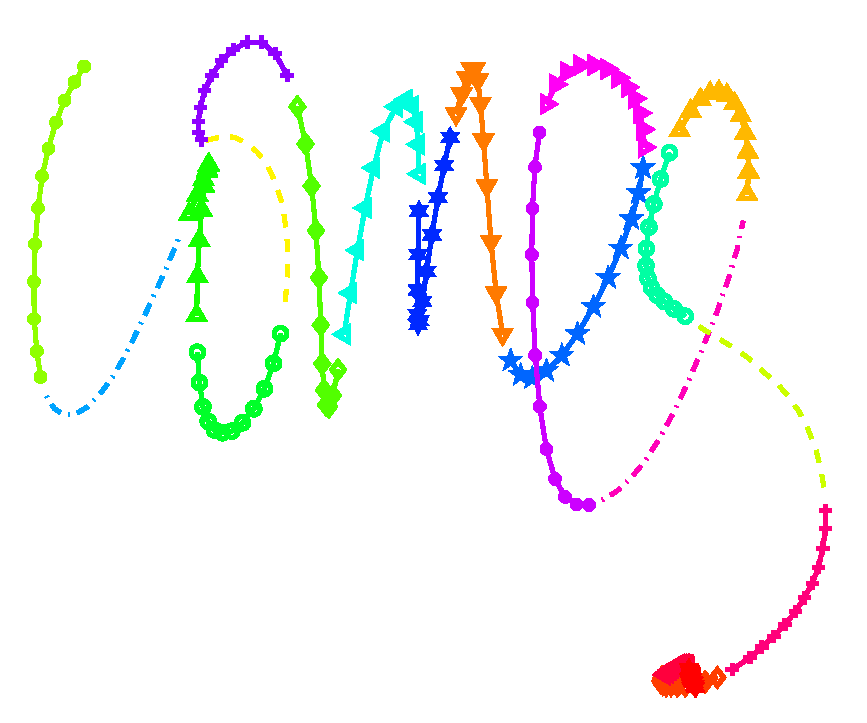
\includegraphics[width=0.22\columnwidth]{./Graphic/Pic_words_forSystemSection/3333_thWord_component.eps}} \\
%\multicolumn{3}{c}{(c) Component extraction for word `comes'} \\
%\multicolumn{3}{c}{ } \\ 
%\end{tabular}
%\caption{{An illustration of %segmented words and their 
%component extraction.
%%(a) shows the separated words from the trajectory in \figref{fig:segmentation}.
%(a)-(c) show the extracted components
%from the word `when', `it', and `comes'. The length of a component is $L_c = 12$ frames and consecutive components share 8 frames, i.e, components start at every 4 frames. }\vspace{-0mm}}\label{fig:segment_component}
%%\end{minipage}
%\end{figure}





%==================================================================
\subsection{Stroke segment-level Feature}


As mentioned above, we construct short, partially overlapped, and fixed-length stroke segments by dividing the word segments of a sample. Let the length of a stroke segment be $L_{ss}$, and the length of a word segment be $L_w$. 
Define the overlapped ratio $r$ to be the number of shared frames between a pair of adjacent stroke segments divided by the stroke segment length $L_{ss}$. Then the $i$-th stroke segment starts at the frame of $(1-r)L_{ss} * i$ and its length is $L_{ss}$. 
This way, we can construct around $\left \lfloor\frac{L_w}{(1-r)L_{ss}}\right \rfloor$ stroke segment for a word segment.
Given a sample that consists of $n$ word segments with length $L^i_{w}, i=1,2,\ldots, n$, respectively, we can in total construct 
$\sum^n_{i=1} \left \lfloor \frac{L^i_w}{(1-r)L_{ss}}\right \rfloor$ stroke segments. 
%Figure~\ref{fig:segment_component} (a)-(c) illustrates the components constructed from three word segments shown in Figure~\ref{fig:segmentation}, with  $L_c = 12$ and $r = 2/3$.



To combine the frame-level features in a stroke segment into a stroke segment-level feature,  we sequentially concatenate the features extracted from all the frames. With 19-dimension feature at frame level, the dimension of this stroke segment-level feature is $19 * L_{ss}$.




 \begin{figure}[!t]
 \vspace{2mm}
 \scriptsize
 \centering
     \begin{tabular}{ m{0.2cm}  m{2.2cm} m{2.2cm} m{2.2cm} }
     \hline
   	   & \textbf{$L_s = 2,000$} & \textbf{$L_s = 4,000$} & \textbf{$L_s = 8,000$} \tabularnewline \hline \hline
     	U1
    & {\includegraphics[width=0.3\columnwidth]{./Graphic/pictures_states/sample2.eps}}
    & {\includegraphics[width=0.3\columnwidth]{./Graphic/pictures_states/para2.eps}}
	& {\includegraphics[width=0.3\columnwidth]{./Graphic/pictures_states/whole2.eps}}\tabularnewline \hline
		U2
    & {\includegraphics[width=0.3\columnwidth]{./Graphic/pictures_states/sample3.eps}}
    & {\includegraphics[width=0.3\columnwidth]{./Graphic/pictures_states/para3.eps}}
	& {\includegraphics[width=0.3\columnwidth]{./Graphic/pictures_states/whole3.eps}}\tabularnewline \hline
\end{tabular}
\vspace{-0mm}
\caption {{style-level features (co-occurrence matrix) extracted from samples of two users. We choose $K=100$ for illustration purpose.
 As the sample length increases, the shape of co-occurrence matrices remain similar, but the value for each element (i.e. the occurrences) increases. The results suggest that the matrices can model handwriting styles.
 }\vspace{-2mm}}\label{tab:sample-para-whole}
\end{figure}

%===================================================================================
\subsection{Style-level Feature}

Simply concatenating all stroke segment-level features of a sample together will create a style feature vector of huge dimensions. For instance, for a sample with $n$ word segments, the dimension of the style feature vector is
$$\sum^n_{i=1} \left \lfloor \frac{L^i_w}{(1-r)L_{ss}}\right \rfloor * 19. $$ 
%
To reduce the dimension of style-level features, we first quantize the stroke segment-level features.
We use training samples to learn stroke segment primitives. Specifically, for each sample, we extract all the stroke segments from all the training samples. % and their stroke segment-level features. 
We then use a $K$-means algorithm to group the stroke segment-level features into $K$ clusters.
The center of each cluster is considered as a primitive of stroke segment-level features. With the $K$ clusters, we achieve a vocabulary with $K$ primitives.
We index these $K$ primitives consecutively from 1 to $K$. With these primitives, we can quantize any stroke segment-level feature, for both the training samples and the testing samples, by finding its nearest primitive and assigning the stroke segment with the index of the corresponding primitive.

We then construct the style-level feature by examining the transition of consecutive stroke segments.  Specifically,
for each pair of sequential stroke segments (with an offset of $(1-r)L_{ss}$ frames in the same word segment), we denote their transition
as an ordered pair $<i,j>$, where $i$ and $j$ are the primitive indices of these two stroke segments. Scanning all such stroke segments pairs
in a sample, we can build a $K\times K$ co-occurrence matrix, in which the $ij$-th element indicates the number of
$<i,j>$ stroke segment transitions in this sample. We finally reshape this matrix into a $K^2$ dimension vector as the feature of this sample.
Figure~\ref{tab:sample-para-whole} shows examples of the constructed style-level features in the form of the co-occurrence matrix, from two users' samples.  
%As the sample length increases, the absolute value for each element (i.e., the occurrences) increases, but the shape of co-occurrence matrices remain similar. This suggest that the matrices can model handwriting styles.
%From \figref{tab:sample-para-whole}, we can observe that the co-occurrence matrix of two users are distinguishable, which indicates the sample level features can represent handwriting styles.



\subsection{Classification}
\label{sec:classification}




We choose SVM~\cite{light-svm} as the classification algorithm, because SVM is relatively efficient and showed accurate classification results in many real-life systems. SVM utilizes a ``kernal trick'' to generalize data well even for high-dimension features. \jingap{In our experiments, we choose the (Gaussian) radial basis function (RBF) kernel. We use grid search method to optimize  RBF SVM parameters $C$ and $\gamma$~\cite{grid-search}, and other parameters are set as default. Finally, we set $\gamma$ as $0.01$ and the penalty parameter $C$ as 5000.  }


For challenge-response authentication, the main goal of the classifier is to verify a user's identity, thus we train multiple binary-class classifiers for all users. \jingap{We split the input data into two parts: training data and testing data. The training data are used to model the writing style of a user, and  testing samples are used to test a user's writing style, thus samples should include writing style representations of the user. Since the writing styles are extracted from stroke segments instead of letters.  Thus, as long as enough stroke segments are used for training and testing samples, MoCRA can model a user's writing style reliably.
We assume the content of the challenge has a fair distribution, so the length of a sample (i.e., how many letters, stroke segments or frames in a sample) indirectly shows the representations of the writing style. We will examine appropriate length in Section~\ref{sec:para}.}

For each user, we take training samples from this user as positive samples and the other users' training samples as negative samples and train a binary SVM classifier. Given a new test sample and the user identity it claims, we test it with the user's binary SVM classifier. The sample will be authorized if the classifier returns a positive response, and be rejected with a negative result. In addition, the classifiers should reject any impostors, the samples of which are never part of the training data.




 


